\subsection{Redux}
This subsystem allows the Client Layer to interact with the HTTP Interface. It will give information to all the different subsystems.

\begin{figure}[h!]
	\centering
 	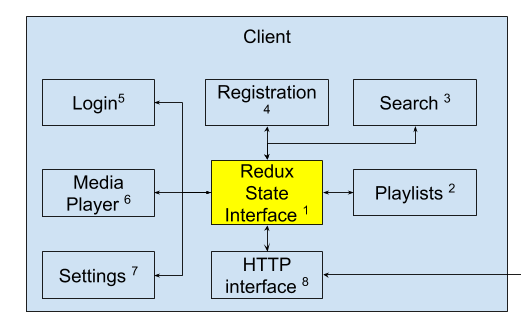
\includegraphics[width=0.60\textwidth]{images/client/client_redux.png}
 	\caption{Redux subsystem}
\end{figure}

\subsubsection{Assumptions}
We are assuming the user is using Google Chrome, and the user does not require any accessibility needs for browsing/searching.

\subsubsection{Responsibilities}
The Redux Interface responsibilities include logging in and registering users, organizing the results from the search, and creating/editing/deleting the playlists from the various third party sources (e.g. Spotify, YouTube).

\subsubsection{Subsystem Interfaces}
\begin {table}[H]
\caption {Redux interfaces} 
\begin{center}
    \begin{tabular}{ | p{1cm} | p{6cm} | p{3cm} | p{3cm} |}
    \hline
    ID & Description & Inputs & Outputs \\ \hline
    \#1 & Playlists & \pbox{3cm}{N/A} & \pbox{3cm}{List of song information from specific Playlist}  \\ \hline
    \#2 & Search & \pbox{3cm}{Search Term} & \pbox{3cm}{Playlists}  \\ \hline
    \#3 & Registration & \pbox{3cm}{E-mail \\ Password \\ Name} & \pbox{3cm}{N/A}  \\ \hline
    \#4 & Login & \pbox{3cm}{E-mail \\ Password} & \pbox{3cm}{N/A}  \\ \hline
    \#5 & Media Player & \pbox{3cm}{ Paused \\ Volume} & \pbox{3cm}{Song Functionality}  \\ \hline
    \#6 & Settings & \pbox{3cm}{N/A} & \pbox{3cm}{Output 1}  \\ \hline
    \end{tabular}
\end{center}
\end{table}

\newpage
